\chapter{Introdução às funções orgânicas}
\begin{mdframed}[backgroundcolor=orange!20,linewidth=0pt,roundcorner=10pt]
	\minitoc
\end{mdframed}
As funções orgânicas são grupos de compostos químicos que compartilham características estruturais e propriedades químicas semelhantes. Elas desempenham um papel fundamental na Química Orgânica, que é o ramo da Química que se concentra no estudo dos compostos que contêm carbono. Os compostos orgânicos podem ser encontrados em uma variedade impressionante de formas e tamanhos, e as funções orgânicas são a maneira pela qual os químicos classificam e compreendem essa diversidade.

As funções orgânicas são essenciais para entender a química dos compostos orgânicos e desempenham um papel crucial em muitos aspectos da química, incluindo a síntese de produtos químicos, a bioquímica, a farmacologia e a indústria química. Esta introdução pretende explorar algumas das funções orgânicas mais comuns e destacará sua importância no estudo da Química Orgânica e na vida cotidiana.


\section{Reconhecimento de padrões}
Faça um exercício mental simples: você consegue separar os bilhões de seres humanos que habitam o planetinha azul chamado Terra de acordo com alguma característica? Analisando friamente, percebemos diferenças no formato dos olhos, na pigmentação da pele, no formato dos cabelos, entre tantas outras características. Se você agrupou alguns humanos, você provavelmente chegou perto de uma etnia. Paramos por aqui com humanos.

Igualmente, se você decidir agrupar automóveis segundo, por exemplo, a potência do motor, número de portas ou qualquer outra característica, você criou uma categoria automobilística.

Este exercício pode ser repetido com músicas, livros, filmes computadores, celulares, ou números, entre tantos outros possíveis elementos que podem ser agrupados.

Fácil, certo?

Sim, desde que você defina alguma característica que diferencie um grupo de outro e coloque junto entidades com características semelhantes.

Antes de tratarmos de moléculas orgânicas, você precisa acostumar seu cérebro naquilo que é conhecido como \textbf{"Reconhecimento de Padrões"}. Veja como nem sempre é simples. oi

\begin{table}[!h]
	\begin{center}
	\caption{\label{padroes}Exercício simples sobre reconhecimento de padrões}
	\vspace{0.5cm}
	\begin{tabular}{|c | c | c|}
	\hline
	4 & 15 & 5\\
	\hline
	5 & 24 & 8\\
    \hline
	2 & 3 & 1\\
	\hline
    7 & \textbf{x} & 16\\
    \hline
	\end{tabular}
	\end{center}
\end{table}

Como você encontra o valor desconhecido apresentado na tabela \ref{padroes}? Existe um padrão que se repete em todas as linhas e caso o encontre nas três primeiras linhas, o valor de x quase que emerge de seu cérebro. 

Quanto tempo levou para encontrar o padrão, principalmente até se dar conta de que pode ignorar a coluna numérica da esquerda?

Independente do tempo gasto na resolução do problema, o padrão escondido nos números é bem simples: os valores numéricos da coluna central são \textbf{o triplo} dos valores da coluna numérica da direita. Assim, o valor de x deve ser o triplo de 16, ou seja, 48.

Existe um outro aspecto que deve ser considerado neste ponto de nossa análise sobre funções orgânicas: a similaridade. De modo bem simplificado, podemos admitir que similaridade está muito relacionada com semelhança e assim podemos dizer que a entidade A é similar à entidade B se vários elementos presentes em A também estejam presentes na entidade B.

Considere a Figura \ref{fig:carros} a seguir. Nela podemos visualizar um conjunto de desenhos com a parte dianteira de alguns automóveis fictícios.

\begin{figure}[h]
	\centering
	\caption{Representação de alguns automóveis.}
	\vspace{0.5cm}
	
\includegraphics[width=0.5\linewidth]{imagens/19035-NRYBNX.jpg}
    \caption*{Fonte: https://shorturl.at/crzG0}
	\label{fig:carros}
\end{figure}

A Figura \ref{fig:carros} neste contexto ajuda a praticar a busca por similaridade em imagens, algo que será muito útil quando precisarmos identificar todas as funções orgânicas presentes em uma molécula polifuncional, pois uma destas funções deve ser a chamada "sênior" ou "principal" para que possamos montar o seu nome a partir de sua estrutura.

Quais elementos tornam as seis partes da imagem representada na figura similares entre si? Podemos visualizar alguns elementos presentes em todas as imagens:

\begin{itemize}
	\item Duas rodas visíveis.
	\item Dois espelhos retrovisores
	\item Um para-brisa
\end{itemize}

Repare que os faróis dos automóveis não são idênticos, assim como as grades frontais também são distintas. Assim, as representações dos automóveis são similares em algum aspecto.

%########################
\section{Função orgânica}
O mesmo ocorrerá quando precisarmos analisar uma estrutura orgânica complexa em busca das funções orgânicas presentes. Veja a molécula representada na Figura \ref{fig:vanco} a seguir.

\begin{figure}[h]
	\centering
	\caption{Estrutura da vancomicina}
	\vspace{0.5cm}
	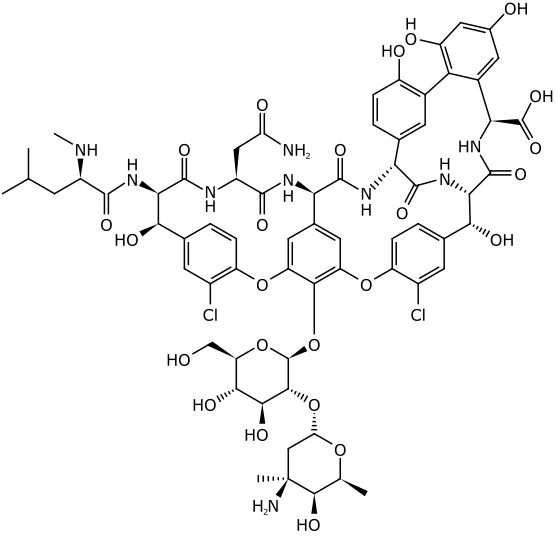
\includegraphics[width=0.85\linewidth]{imagens/557px-Vancomycin.svg}
	\caption*{Fonte: Wikipedia https://shorturl.at/nAZ01}
	\label{fig:vanco}
\end{figure}

Ainda sem analisar os detalhes de cada função orgânica presente na vancomicina, uma substância classificada como antibiótico, percebe-se que existem alguns conjuntos de átomos que se repetem na estrutura, algo como (guardadas as devidas proporções) ocorre na Figura \ref{fig:carros}.

É relativamente fácil encontrar alguns desses grupos de átomos:

\begin{itemize}
	\item átomo de Oxigênio ligado a átomo de Hidrogênio;
	\item átomo de Nitrogênio ligado a dois átomos de Oxigênio;
	\item átomo de Carbono ligado a um átomo de Oxigênio por uma ligação covalente dupla.
\end{itemize}

Cada um desses conjuntos é uma \textbf{função orgânica}.

Existem dezenas delas, todas categorizadas, organizadas e designadas por seus nomes pela IUPAC, conforme pode ser analisado no IUPAC BlueBook \cite{iupac2013}.

O número de substâncias orgânicas conhecidas já ultrapassou a grandeza de dezenas de milhões, e métodos sintéticos novos geram ainda mais substâncias \cite{doi:10.1021/acs.jmedchem.2c00223}. Cada substância química precisa de um nome que caracterize sua unicidade e existem muitas regras para que cada uma delas tenha seu nome de maneira inequívoca.

A Figura \ref{fig:funcoes2} mostra um resumo das funções orgânicas que serão analisadas neste livro, contendo, além do nome, uma representação geral e também o sufixo correspondente.

\begin{figure}[h]
	\centering
	\caption{Resumo das funções orgânicas.}
	\vspace{0.5cm}
	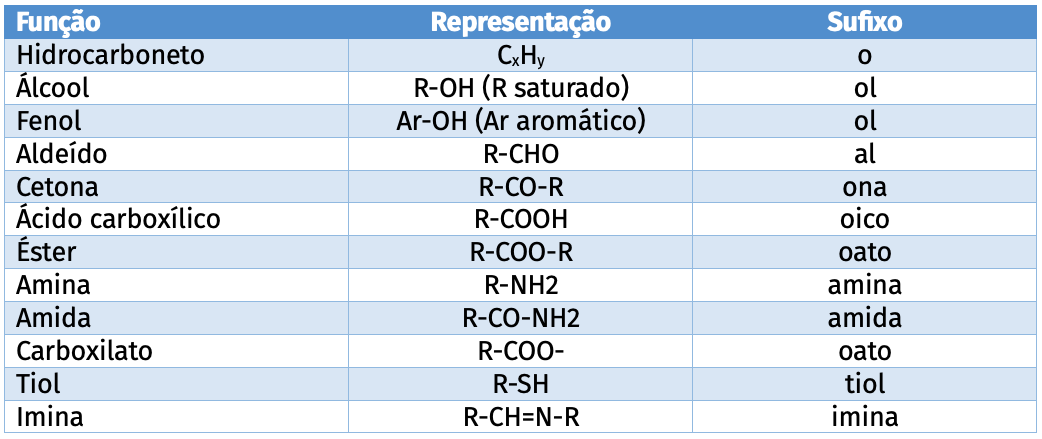
\includegraphics[width=1\linewidth]{imagens/funcoes.png}
	\caption*{Fonte: autores}
	\label{fig:funcoes2}
\end{figure}

%###################################
